\newgeometry{top=5cm}

\section{\red{Exhibit Commands Usage Examples (Remove This Section in Final Submission)}}

\vspace{5mm}
\textbf{1. Create a cover page for an exhibit}
\begin{verbatim}
\refexhibitlabel{cv}

\includepdf[pages=-]{cv.pdf}
\end{verbatim}
where "cv" is the label in the index\_of\_exhibits.tex, "cv.pdf" is under exhibits/. It will create a cover page followed by the cv.pdf.

Define pages to be included:

\begin{itemize}
    \item All pages
        \begin{verbatim}
        
\includepdf[pages=-]{cv.pdf}
        \end{verbatim}
    \item One page (1st page)
        \begin{verbatim}
        
\includepdf[pages=1]{cv.pdf}
        \end{verbatim}
    \item Range ([2,3])
        \begin{verbatim}
        
\includepdf[pages=2-3]{cv.pdf}
        \end{verbatim}
    \item Some pages
        \begin{verbatim}
        
\includepdf[pages={1,2}]{cv.pdf}
        \end{verbatim}    
\end{itemize}

\vspace{5mm}
\textbf{2. Create a cover page for a parent exhibit and some child exhibits}
\begin{verbatim}
\refexhibitlabel{3}

\refexhibitsublabel{ms-in-cs}

\refexhibitsublabel{ms-in-cs-gpa}


\includepdf[pages=-]{ms-in-cs.pdf}

\includepdf[pages=-]{ms-in-cs-gpa.pdf}
\end{verbatim}
where "3", "ms-in-cs", and "ms-in-cs-gpa" are the labels in the index\_of\_exhibits.tex, "ms-in-cs.pdf" and "ms-in-cs-gpa.pdf" are under exhibits/. It will create a cover page followed by the two pdf files. \red{Note the space between `refexhibitlabel` and refexhibitsublabel.}

\refexhibitlabel{3}

\refexhibitsublabel{ms-in-cs}

\refexhibitsublabel{ms-in-cs-gpa}


\includepdf[pages=-]{ms-in-cs.pdf}


\includepdf[pages=-]{ms-in-cs-gpa.pdf}

More examples are coming below.
%%%%%%%%%%%%%%%%%%%%%%%%%%%%%%%%%%%%%%%%%%%%%%%%%%%%%%%%%
\refexhibitlabel{rl-prof-someone}

\includepdf[pages=-]{recommendation-letter.pdf}

\refexhibitlabel{white-house-list}

\includepdf[pages=-]{white-house-list.pdf}

\refexhibitlabel{Dhanasar}
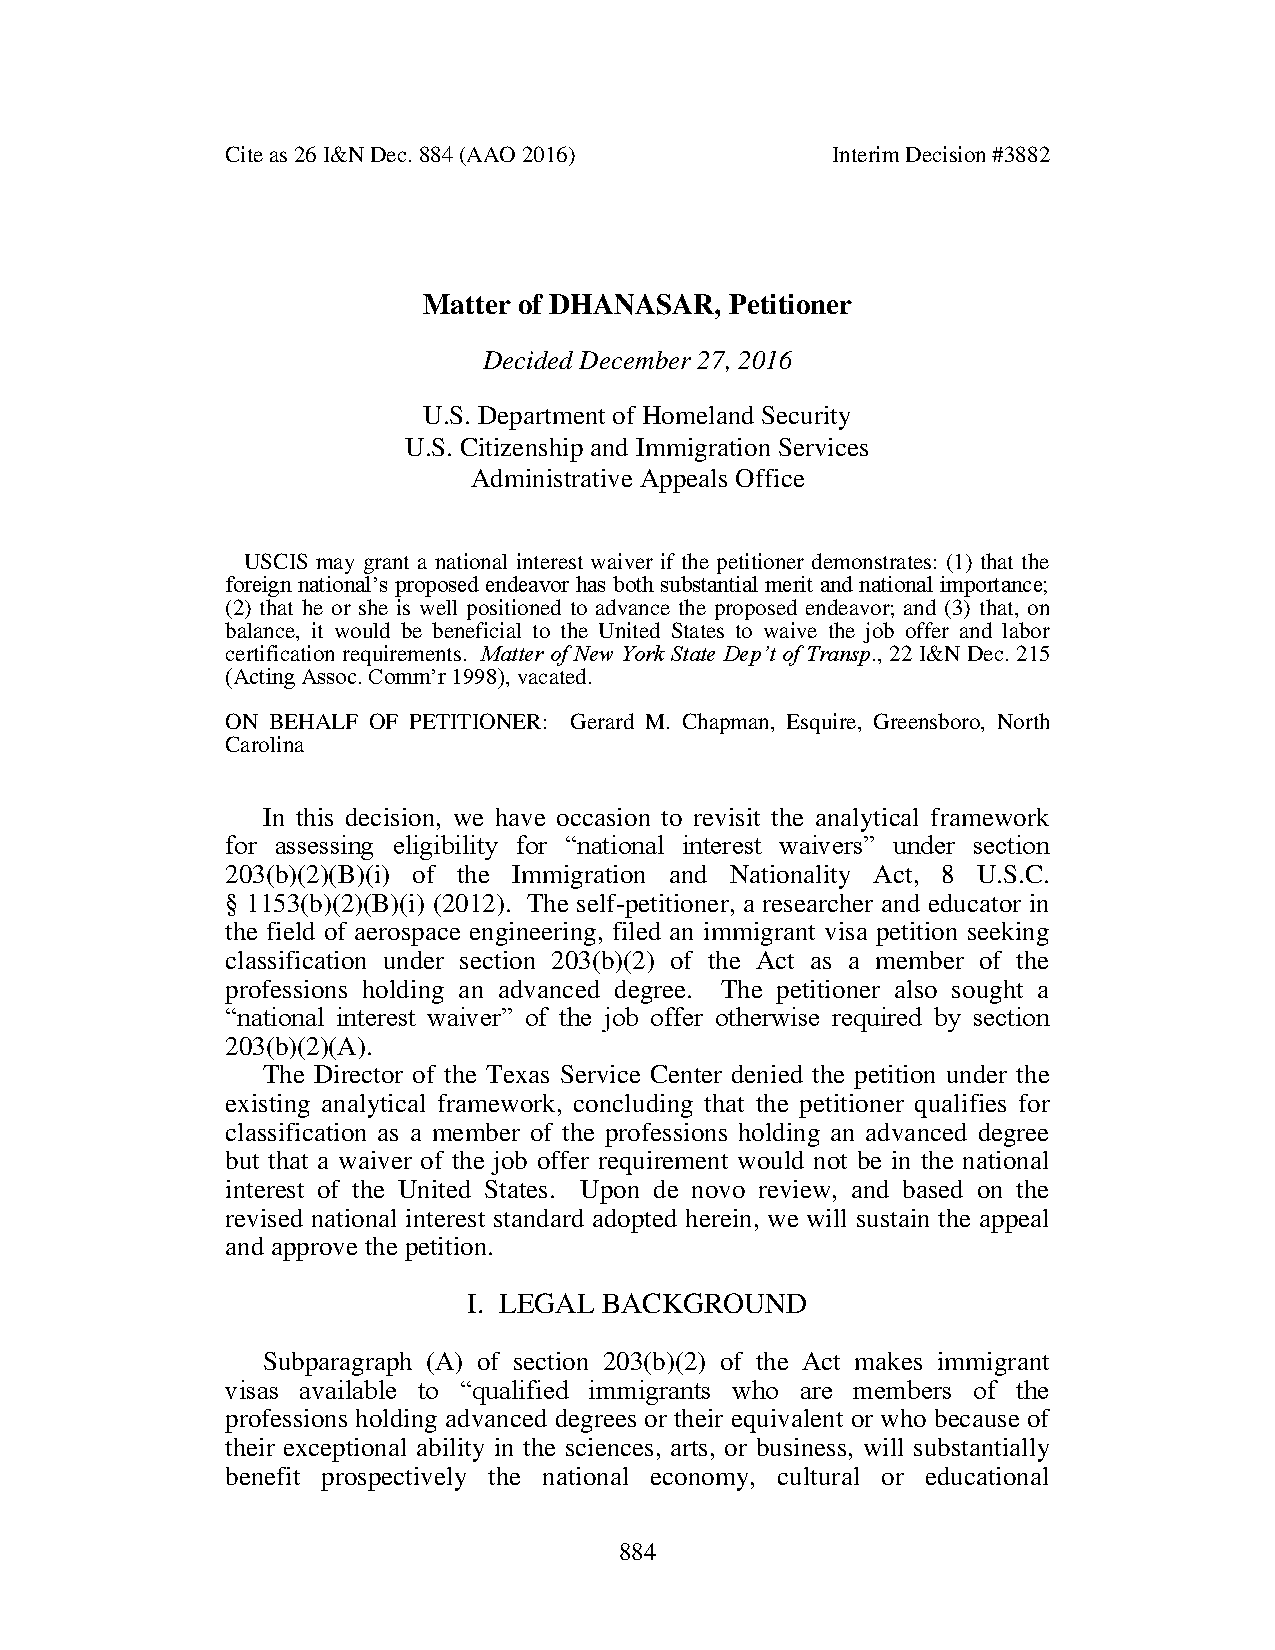
\includepdf[pages=-]{Dhanasar.pdf}

\restoregeometry